\section{Life Cycle Of Software}
\subsection{Whats's Life Cycle Of Software?}
As the name suggest it's the life cycle of a software from start to finish , life cycle also known as model is a methodology
that serves to help developers in building their product , each life cycle has steps and a chronology to follow

\subsection{Waterfall Life Cycle}
The Waterfall Model is considered one of the first software development methodologies for large-scale 
projects. As the name suggests, it follows a series of sequential steps, one after the other, similar to a waterfall. This model
formed the basis of early software life cycles, solving many issues but also introducing some new challenges. Over time, 
other life cycle models were developed and improved upon.

\subsubsection{First Version}
The first version of the WaterFall model includes 5 steps

\begin{itemize}
    \item \textbf{Definition \& Needs Analysis}: The first step involves interacting with the client to understand their 
    requirements and guide them. This step is crucial because any misunderstanding between the developers and the client 
    could cause the entire project to fail, requiring a restart. The output of this step is a document that contains all
    the necessary information, called the "Requirements Document."
    
    \item \textbf{Design}: In this step, developers create the software's architecture, defining the modules and how they
    interact with each other. The output of this step is the "Design Document."
    
    \item \textbf{Coding}: The implementation of the modules into a programming language takes place in this step.
    
    \item \textbf{Testing}: This step involves testing the software and fixing bugs.
    
    \item \textbf{Deployment \& Maintenance}: The final step is delivering the software to the client and maintaining it 
    by adding new features and fixing undetected and future bugs.
\end{itemize}

\vspace{0.5cm}
\begin{center}
\begin{tikzpicture}
    \draw (-1,0) rectangle (3.5,1.5);
    \node at (1.25,0.75) {Definition \& Needs Analysis};

    \draw[->] (3.5,0.75) -- (5,0.75) -- (5,0);
    \node at (5.5,1) {Requirements Document};

    \draw (4,-1.5) rectangle (6,0);
    \node at (5,-0.75) {Design};

    \draw[->] (6,-0.75) -- (7.5,-0.75) -- (7.5,-1.5);
    \node at (7.5,-0.5) {Design Document};

    \draw (6.5,-3) rectangle (8.5,-1.5);
    \node at (7.5,-2.25) {Coding};

    \draw[->] (8.5,-2.25) -- (10,-2.25) -- (10,-3);
    \node at (10.15,-2) {Software's Modules};

    \draw (9,-4.5) rectangle (11,-3);
    \node at (10,-3.75) {Testing};

    \draw[->] (11,-3.75) -- (13.75,-3.75) -- (13.75,-4.5);
    \node at (12.5,-3.5) {Software};

    \draw (11.5,-6) rectangle (16,-4.5);
    \node at (13.75,-5.25) {Deployment \& Maintenance};
\end{tikzpicture}
\end{center}

\subsubsection{Improved Version}
The Waterfall model was slightly improved by dividing some steps into two:
\begin{itemize}
    \item \textbf{Design}:
        \begin{itemize}
            \item \textbf{Architectural Design}: Design how the software's modules will interact with each other.
            \item \textbf{Detailed Design}: Design each module's components in detail.
        \end{itemize}
    \item \textbf{Testing}:
        \begin{itemize}
            \item \textbf{Unit Testing}: Test all the modules independently.
            \item \textbf{Integration Testing}: Test the interaction and communication between modules.
        \end{itemize}
\end{itemize}

\vspace{2.5cm}
\begin{center}
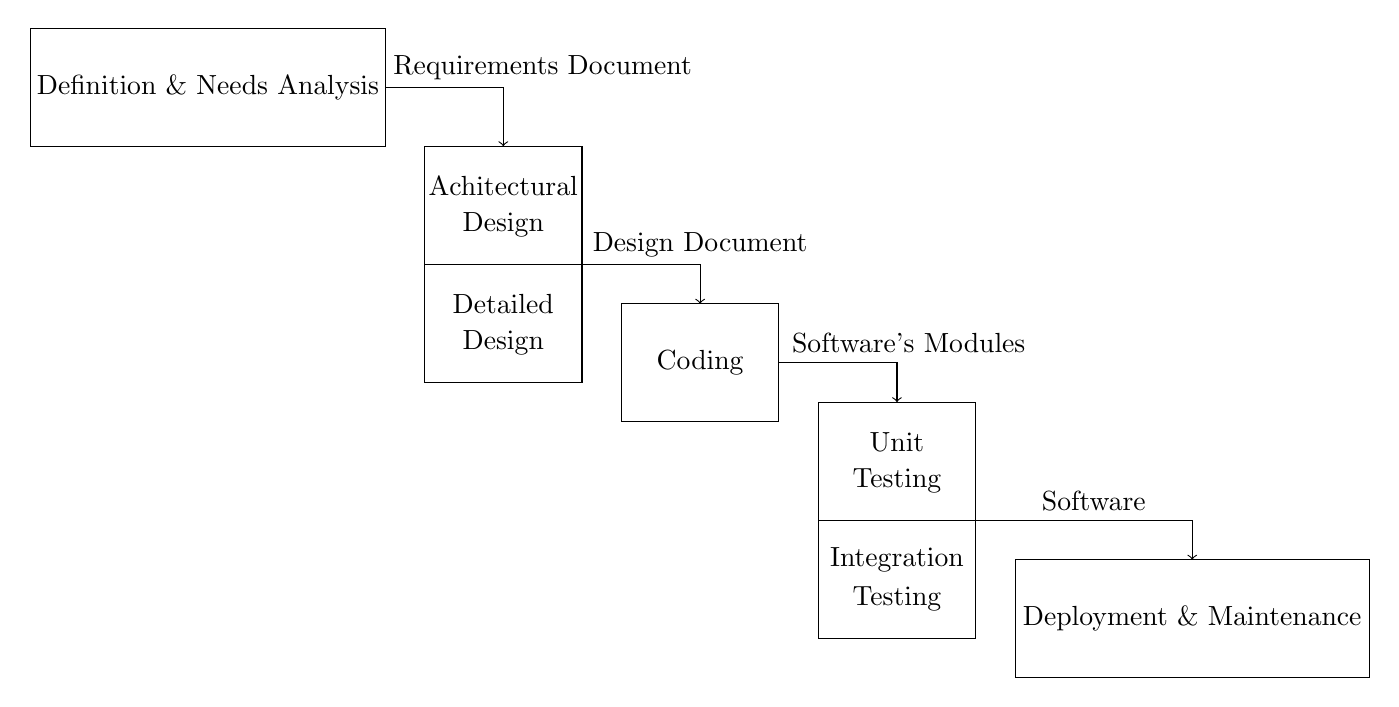
\begin{tikzpicture}
    \draw (-1,0) rectangle (3.5,1.5);
    \node at (1.25,0.75) {Definition \& Needs Analysis};

    \draw[->] (3.5,0.75) -- (5,0.75) -- (5,0);
    \node at (5.5,1) {Requirements Document};

    \draw (4,-1.5) rectangle (6,0);
    \node at (5,-0.5) {Achitectural};
    \node at (5,-1){Design};
    \draw (4,-3) rectangle (6,-1.5);
    \node at (5,-2) {Detailed};
    \node at (5,-2.5) {Design};

    \draw[->] (6,-1.5) -- (7.5,-1.5) -- (7.5,-2);
    \node at (7.5,-1.25) {Design Document};
    
    \draw (6.5,-3.5) rectangle (8.5,-2);
    \node at (7.5,-2.75) {Coding};

    \draw[->] (8.5,-2.75) -- (10,-2.75) -- (10,-3.25);
    \node at (10.15,-2.5) {Software's Modules};
    
    \draw (9,-4.75) rectangle (11,-3.25);
    \node at (10,-3.75) {Unit};
    \node at (10 ,-4.25){Testing};

    \draw (9,-6.25) rectangle (11,-4.75);
    \node at (10,-5.25) {Integration};
    \node at (10,-5.75) {Testing};

    \draw[->] (11,-4.75) -- (13.75,-4.75) -- (13.75,-5.25);
    \node at (12.5,-4.5) {Software};

    \draw (11.5,-6.75) rectangle (16,-5.25);
    \node at (13.75,-6) {Deployment \& Maintenance};
\end{tikzpicture}
\end{center}

\vspace{1cm}

\begin{prettyBox}{Note}{red}
    \textbf{Why Architectural Design before Detailed Design?} \\
 
    We first define the high-level structure of the modules and their interactions to provide an overall system architecture.
    This gives a clear overview of the software before delving into the detailed characteristics of each module.\\

    \textbf{Why Unit Testing before Integration Testing?} \\

    It is important to test each module individually to ensure that they function correctly in isolation. This helps to simplify debugging, as any issues can be pinpointed within a module, rather than confusion over whether the problem lies in the module itself or in the interaction between modules.
\end{prettyBox}

\subsubsection{Pros}
\begin{itemize}
    \item Helps organize the project by providing a clear structure and well-defined stages.
    \item Simple to understand and execute, especially for small to medium-sized projects.
    \item Easy to manage due to its linear progression, making it suitable for projects with stable requirements.
    \item Documentation is thorough, ensuring that each phase has a clear output.
\end{itemize}

\subsubsection{Cons}
\begin{itemize}
    \item Lack of parallelism, as tasks cannot be done concurrently, leading to longer project timelines.
    \item High dependency between steps, meaning each phase must be completed fully before the next can begin.
    \item Inflexibility to handle changes during development, as going back to previous phases can be costly and time-consuming.
    \item Risk of significant rework if the needs analysis phase is not done properly, potentially requiring a restart from the beginning.
    \item Limited feedback during development, as testing and validation occur only at later stages.
\end{itemize}


\vspace{1cm}
\subsection{V Life Cycle}
The V Model is similar to the Waterfall Model, as both follow a sequential process with the same key steps. However, 
the V Model introduces a key difference: it integrates preparation for the corresponding testing phases alongside each 
development step, forming a "V" shape in the process diagram.
For example, after completing the \textbf{Architectural Design}, preparation for \textbf{Integration Testing} begins. 
Similarly, after the \textbf{Detailed Design}, preparation for \textbf{Unit Testing} takes place. This parallel preparation
ensures better alignment between development phases and their corresponding testing phases, saving time and helping to catch 
potential issues earlier.
\vspace{1cm}
\begin{center}
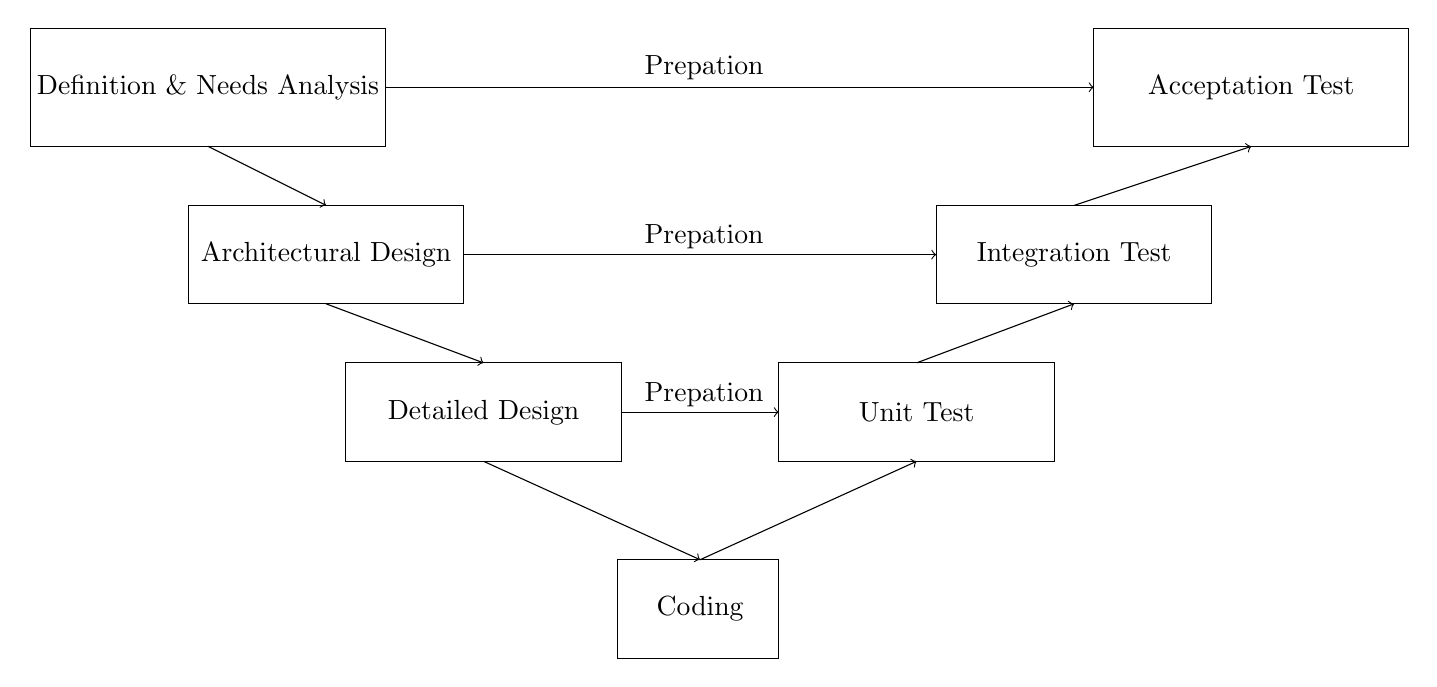
\begin{tikzpicture}
    \draw (-1,0) rectangle (3.5,1.5);
    \node at (1.25,0.75) {Definition \& Needs Analysis};

    \draw[->] (3.5,0.75) -- (12.5,0.75);
    \node at (7.55,1) {Prepation};
    \draw[->] (1.25,0) -- (2.75,-0.75);

    \draw (1,-2) rectangle (4.5,-0.75);
    \node at (2.75,-1.375) {Architectural Design};

    \draw[->] (4.5,-1.375) -- (10.5,-1.375) ;
    \draw[->] (2.75,-2) -- (4.75,-2.75);
    \node at (7.55,-1.15) {Prepation};

    \draw (3,-4) rectangle (6.5,-2.75);
    \node at (4.75,-3.375) {Detailed Design};

    \draw[->] (6.5,-3.375) -- (8.5,-3.375);
    \node at (7.55,-3.15) {Prepation};
    \draw[->] (4.75,-4) -- (7.5,-5.25);
    
    \draw (6.45,-6.5) rectangle (8.5,-5.25);
    \node at (7.5,-5.875) {Coding};

    \draw[->] (7.5,-5.25) -- (10.25,-4);
    
    \draw (8.5,-4) rectangle (12,-2.75);
    \node at (10.25,-3.375) {Unit Test};

    \draw[->] (10.25,-2.75) -- (12.25,-2);
    
    \draw (10.5,-2) rectangle (14,-0.75);
    \node at (12.25,-1.375) {Integration Test};

    \draw[->] (12.25,-0.75) -- (14.5,0);
    
    \draw (12.5,0) rectangle (16.5,1.5);
    \node at (14.5,0.75) {Acceptation Test};


\end{tikzpicture}
\end{center}

\vspace{1cm}
\begin{prettyBox}{Note}{red}
 It's important to note that while there is parallelism in the preparation for testing, the development steps themselves are 
still executed sequentially, with no overlap.  
\end{prettyBox}

\vspace{0.5cm}
\subsubsection{Pros}
\begin{itemize}
    \item Improves time efficiency by preparing testing phases in parallel with development phases, allowing for faster transitions between steps.
    \item Allows early detection of potential issues, as test preparation begins immediately after design, enabling a quicker response to design flaws or misunderstandings.
\end{itemize}

\subsubsection{Cons}
\begin{itemize}
    \item Lacks parallelism in the execution of development steps, as each phase must still be completed sequentially.
    \item Carries the risk of significant rework if the needs analysis phase is not thoroughly completed, potentially requiring a restart from the beginning.
    \item Maintains strong dependencies between steps, meaning that each phase relies heavily on the correct execution of the previous one. This can create delays or issues if earlier phases were not executed properly.
\end{itemize}

\vspace{1cm}
\subsection{Prototyping Life Cycle}
The Prototyping Life Cycle was developed to reduce the risk of restarting the project due to incomplete, contradictory, 
or ambiguous requirements in the initial requirement document. 
In this approach, the development team first meets with the client to conduct a needs analysis and create the initial 
requirement document. Then, a small prototype is developed and presented to the client for feedback. This process helps
clarify the client's needs, improve understanding, and refine the requirements document. 
The cycle of developing and reviewing prototypes continues until the requirements document is fully defined and clear. 
Once finalized, the project proceeds through the remaining steps of the chosen life cycle model.


\vspace{0.5cm}
\begin{prettyBox}{Should We Discard the Prototype or Build Upon It?}{red}
    The decision depends on several factors. If the prototype was quickly assembled and lacks scalability or if adding 
    new features proves to be complex due to a poorly thought-out design, it might be more efficient to discard the
    prototype and start fresh.\\

    However, if the prototype was designed with a solid foundation and can easily accommodate additional features,
    continuing to build on it could save time and resources.
\end{prettyBox}

\vspace{1.5cm}
\begin{center}
    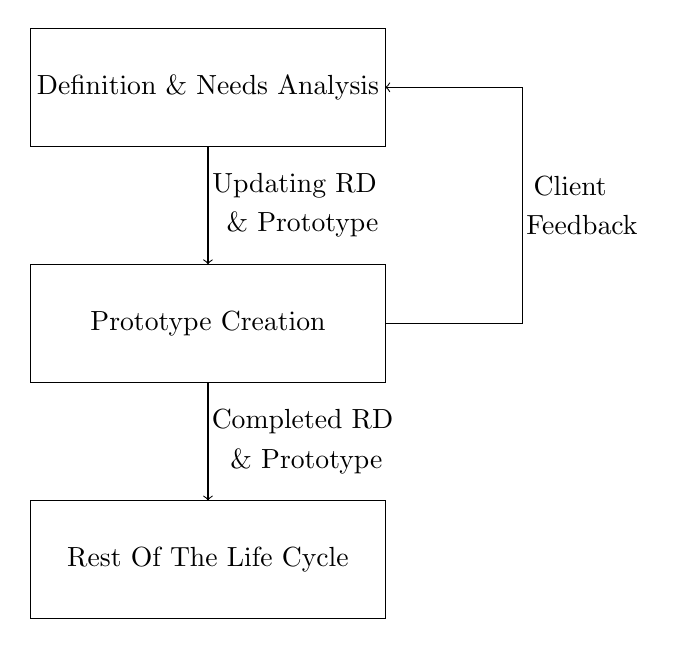
\begin{tikzpicture}
    \draw (-1,0) rectangle (3.5,1.5);
    \node at (1.25,0.75) {Definition \& Needs Analysis};
 
    \draw[->] (1.25,0) -- (1.25,-1.5);
    \node at (2.35,-0.5) {Updating RD};
    \node at (2.45,-1) {\& Prototype};

    \draw (-1,-3) rectangle (3.5,-1.5);
    \node at (1.25,-2.25) {Prototype Creation};

    \draw[->] (3.5,-2.25) -- (5.25,-2.25) -- (5.25,0.75) -- (3.5,0.75);
    \node at (5.85,-0.5) {Client};
    \node at (6,-1) {Feedback};
    \draw[->] (1.25,-3) -- (1.25,-4.5);
    \node at (2.45 , -3.5) {Completed RD};
    \node at (2.5,-4){\& Prototype};
    \draw (-1,-6) rectangle (3.5,-4.5);
    \node at (1.25,-5.25) {Rest Of The Life Cycle};
    \end{tikzpicture}
\end{center}

\vspace{1cm}
\subsubsection{Pros}
\begin{itemize}
    \item Reduces the risk of restarting the project due to continuous client feedback, as a complete requirements
document is established upfront.
\end{itemize}

\subsubsection{Cons}
\begin{itemize}
    \item Creates uncertainty about whether to discard the prototype or continue building on it, which can be time-consuming 
and resource-intensive.
    \item Carries the cons of the used life cycle
\end{itemize}

\vspace{1cm}
\subsection{Incremental Life Cycle}
The Incremental Life Cycle is an iterative model designed to address the uncertainty of whether to discard the prototype or
continue building on it. 
In this model, development starts with the implementation of a core set of essential features, known as the core increment or
the first increment. This initial increment is delivered to the user for feedback. 
Subsequent increments, each containing additional features, are built on top of the core increment and are also sent to the 
client for review. This process continues iteratively, with feedback shaping the development, until the project is fully completed.

\vspace{0.5cm}

\begin{prettyBox}{Importance Of Selecting The Core Features}{red}
    It is crucial to carefully select the first set of features when implementing the core increment. If this initial set
    is not scalable, it will be difficult for developers to add new features and continue building upon it effectively.
\end{prettyBox}

\vspace{2cm}
\begin{center}
    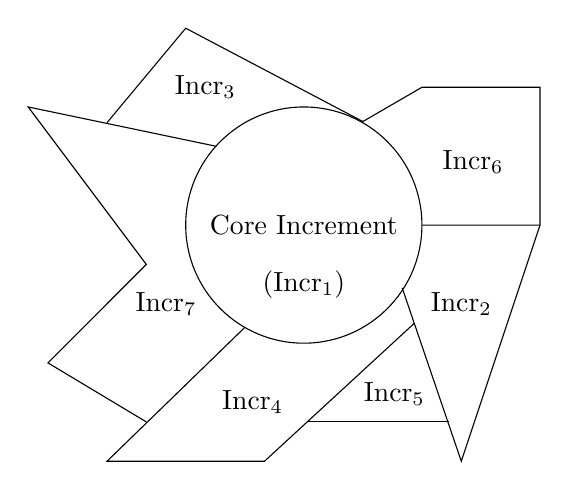
\begin{tikzpicture}
        \draw (0,0) circle[radius = 1.5cm] node {Core Increment};
        \node at (0,-0.75){(Incr$_{1}$)}; 
        \draw (1.5,0) -- (3,0) -- (2,-3) -- (1.25,-0.8);
        \node at (2,-1){Incr$_{2}$}; 
        \draw (0.75,1.315) -- (-1.5,2.5) -- (-2.5,1.3);
        \node at (-1.25,1.75){Incr$_{3}$}; 
        \draw (1.4,-1.25) -- (-0.5,-3) -- (-2.5,-3) -- (-0.75,-1.3); 
        \node at (-0.65,-2.25){Incr$_{4}$}; 
        \draw (0.050,-2.5) -- (1.85,-2.5); 
        \node at (1.15,-2.15){Incr$_{5}$}; 
        \draw (3,0) -- (3,1.75) -- (1.5,1.75) -- (0.75,1.315);
        \node at (2.15,0.8){Incr$_{6}$}; 
        \draw (-2,-2.5) -- (-3.25,-1.75) -- (-2,-0.5) -- (-3.5 , 1.5) -- (-1.11,1);
        \node at (-1.75,-1){Incr$_{7}$}; 
    \end{tikzpicture}
\end{center}

\subsubsection{Pros}
\begin{itemize}
    \item Dividing the project into smaller sets of features makes it easier for developers to manage and focus on one
increment at a time.
    \item Constant client feedback throughout the development process ensures that adjustments can be made as new
features are added.
    \item Minimizes the risk of wasted effort, as nothing is discarded—each increment builds upon the previous one.
\end{itemize}

\subsubsection{Cons}
\begin{itemize}
    \item There is a risk of restarting the project if the developers do not select the right initial set of features for the
core increment, as future increments depend on this foundation.
    \item Each increment inherits the flaws or limitations of the chosen life cycle model.
\end{itemize}

\vspace{1cm}
\subsection{Spiral Life Cycle} The Spiral Life Cycle is an iterative model designed for large-scale projects, with a strong
focus on risk assessment and mitigation throughout the development process. It is called "spiral" because it involves multiple
phases arranged in a spiral pattern, with each loop in the spiral representing a phase of the software development process
(an iteration).

\begin{itemize} 
    \item \textbf{Planning(Objective)}: The project’s objectives are identified, and alternatives and constraints are defined. 
High-level requirements gathering (Needs Analysis) is also performed.
    \item \textbf{Risk Analysis(Risk Management)}: This phase focuses on evaluating risks, uncertainties, and potential problems of the current
iteration, ensuring that risks and strategies to mitigate them are identified early on.
    \item \textbf{Engineering (Development \& Testing)}: The actual designing, development, and testing of the product occur in
this phase, which includes activities such as unit testing and integration testing.
    \item \textbf{Evaluation(Planning next itteration)}: After each iteration (loop) of the spiral, there’s an evaluation of the product by the customer
or stakeholders. Feedback is collected, and necessary changes are made before the next loop begins, allowing for continuous
improvement throughout the project.
\end{itemize}
\begin{center}
\begin{tikzpicture}
   \draw[->] (-6,0) -- (6,0);
   \draw[->] (0,-6) -- (0,6);
   
   \node at (5,5.5){1.Planning};
   \node at (-5,5.5){2.Risk Management};
   \node at (-5.5,-5.5){3.Engineering};
   \node at (5,-5.5){4.Evaluation};

   \draw[domain=0:6.28*5, variable=\t, samples=500, smooth] 
        plot ({\t r}: {0.15*\t});
\end{tikzpicture}
\end{center}
\vspace{1cm}
\subsubsection{Pros}
\begin{itemize} 
\item Continuous client feedback facilitates timely adjustments and improvements to the project.
\item Regular identification and assessment of risks, along with strategies for mitigation, help ensure a smoother development
process. 
\end{itemize}
\subsubsection{Cons}
\begin{itemize} 
\item The model can be complex and challenging to implement effectively, requiring careful planning and coordination.
\item It can be resource-intensive, potentially demanding significant time and effort from the development team.
\end{itemize}
\vspace{1cm}
\subsection{Hybrid Life Cycle}
The Hybrid Life Cycle involves dividing the project into \( n \) parts, where each part$_{i}$ follows its corresponding
lifeCycle$_{i}$ .This model provides the greatest flexibility among all the methodologies discussed so far.
\vspace{1cm}
\begin{center}  
\begin{tikzpicture}
    \draw (2.5,0) rectangle (7,1.5);
    \node at (4.75,0.75) {The Project};
   
    \draw [->] (4.75,0) -- (4.75 , - 1.5) -- (4.75 , -2.5);
    \draw [->] (4.75,-1.5) -- (-4.75,-1.5) -- (-4.75,-2.5);
    \draw [->] (4.75 , -1.5) -- (14.75,-1.5) -- (14.75,-2.5);

    \draw (-6,-4) rectangle (-3.5,-2.5);
    \node at (-4.75,-3.25) {Part$_{1}$};

    \draw [->] (-4.75,-4) -- (-4.75,-7.5);
    
    \draw (-6,-9) rectangle (-3.5,-7.5);
    \node at (-4.75,-8.25) {Life Cycle$_{1}$};

    \draw[dash pattern=on 1pt off 3pt, line width=1pt] (-2.75,-3.25) -- (2.75,-3.25);

    \draw (3.5,-4) rectangle (6,-2.5);
    \node at (4.75,-3.25) {Part$_{5}$};
    
    \draw [->] (4.75,-4) -- (4.75,-7.5);
    
    \draw (3.5,-9) rectangle (6,-7.5);
    \node at (4.75,-8.25) {Life Cycle$_{5}$};


    \draw[dash pattern=on 1pt off 3pt, line width=1pt] (6.75,-3.25) -- (12.75,-3.25);

    \draw (13.5,-4) rectangle (16,-2.5); 
    \node at (14.75,-3.25) {Part$_{n}$};
  
    \draw [->] (14.75,-4) -- (14.75,-7.5);
  
    \draw (13.5,-9) rectangle (16,-7.5);
    \node at (14.75,-8.25) {Life Cycle$_{n}$};

\end{tikzpicture}
\end{center}

\vspace{1cm}

\begin{prettyBox}{Difference Between Incremental \& Spiral \& Hybrid ?}{red}
\begin{itemize}
    \item Hybrid: This model divides the project into \( n \) parts, each with its own life cycle. One of these life cycles
can be Incremental or Spiral.
\item Incremental: This approach breaks the project into a set of features called increments, building each subsequent
increment on the core increment.
\item Spiral: The Spiral model follows an iterative loop structure, where each loop consists of four steps: Planning,
Risk Analysis, Development \& Testing, and Evaluation.
\end{itemize}
\end{prettyBox}

\subsubsection{Pros}
\begin{itemize} 
\item Offers significant flexibility since each part can adopt a different life cycle model tailored to its specific needs
and requirements, enabling teams to capitalize on the strengths of various methodologies.
\end{itemize}
\subsubsection{Cons}
\begin{itemize}
\item Can be complex to manage, as coordinating different life cycles for various parts of the project may require additional
resources and effort.
\item Potential for misalignment between parts if communication and integration aren’t carefully managed, which could lead
to inconsistencies in the overall project.
\end{itemize}

\vspace{1cm}
\begin{prettyBox}{Difference Between The Life Cycles ?}{red}
All the life cycles we've reviewed so far include similar steps (activities), the differences arise in the logical and
chronological sequencing of these activities.
\end{prettyBox}

